\documentclass[11pt]{article}
\usepackage[margin=1in]{geometry}
\usepackage{amsmath}
\usepackage{booktabs}
\usepackage{graphicx}

\title{Step 5 Validation Protocol: Temperature and Field Scans}
\author{}
\date{}

\begin{document}
\maketitle

\section{Purpose of the test}
Step 4 showed that discrete temperature and field controls can separate a
lattice-driven channel from a finite local spin-correlation control.  Step 5
turns that logic into continuous scans.  The test asks whether finite-window
spectral observables follow the phenomenological spin-Peierls order parameter
$\delta(T,B)$ and its associated dynamical lattice coupling
$g_Q^{\mathrm{eff}}$, rather than merely reflecting the presence of a finite
$C_1(T,B)$.

\section{Physical model}
The Hamiltonian is unchanged from Step 4:
\begin{equation}
H_{\mathrm{mix}} =
V_{BD}^{\mathrm{static}} L_{BD}
+ g_Q^{\mathrm{eff}} Q L_{BD},
\end{equation}
with
\begin{equation}
V_{BD}^{\mathrm{static}} =
V_0 + \lambda_\delta \delta(T,B) + \lambda_C C_1(T,B).
\end{equation}
For the lattice scans,
\begin{equation}
g_Q^{\mathrm{eff}} = g_{Q0}
\frac{\delta(T,B)}{\delta(T_{\mathrm{ref}},B_{\mathrm{ref}})}.
\end{equation}
For the $C_1$ static scan, $g_Q^{\mathrm{eff}}=0$ and the scalar
spin-correlation channel is kept active.

\section{Trend definitions}
The spin-Peierls transition temperature is
\begin{equation}
T_{\mathrm{SP}}(B)=
\max\left[0,T_{\mathrm{SP},0}(1-\alpha_B B^2)\right].
\end{equation}
The dimerisation follows
\begin{equation}
\delta(T,B)=
\begin{cases}
\delta_0\left(1-T/T_{\mathrm{SP}}(B)\right)^\beta,
& T<T_{\mathrm{SP}}(B),\\
0, & T\ge T_{\mathrm{SP}}(B).
\end{cases}
\end{equation}
The local spin-correlation proxy remains finite above the transition and is
therefore not treated as an order parameter.

\section{Numerical procedure}
Three scan families are generated:
\begin{center}
\begin{tabular}{llll}
\toprule
Family & Varied parameter & Fixed condition & Channel \\
\midrule
Temperature lattice & $T$ & $B=0$ & dynamic lattice \\
Field lattice & $B$ & $T=7$ & dynamic lattice \\
Temperature $C_1$ & $T$ & $B=0$ & static $C_1$ \\
\bottomrule
\end{tabular}
\end{center}
Each run saves the rephasing real spectrum, raw complex response arrays, and
text/JSON summaries.  The Phase 2 analysis extracts finite-window integrals
around the hybridized diagonal and cross resonances.

\section{Acceptance criteria}
The temperature lattice scan should show the lattice parameters
$\delta(T,0)$ and $g_Q^{\mathrm{eff}}(T,0)$ decreasing to zero at and above
$T_{\mathrm{SP}}$.  The spectral observables do not need to be perfectly
monotonic because peak positions, finite windows, and linewidth effects all
contribute, but a clear regime change should be visible across the transition.

The field scan should suppress the lattice channel as $T_{\mathrm{SP}}(B)$ is
driven below the fixed temperature.  The $C_1$ static scan is not expected to
vanish at $T_{\mathrm{SP}}$; persistence in that control is evidence that a
surviving feature is not unique to the dimerised phase.

\section{Requested figures and data}
Phase 2 should produce:
\begin{itemize}
\item a scan-metrics table with one row per run;
\item trend plots for the temperature lattice, field lattice, and temperature
$C_1$ static scans;
\item a comparison between lattice-dynamic and $C_1$-static temperature scans;
\item a text validation outcome and this updated protocol.
\end{itemize}

\section{Interpretation of possible failures}
If the lattice scan does not show a clear change at the transition, the
finite-window metric may be too insensitive, the scan may need a finer grid near
$T_{\mathrm{SP}}$, or the chosen $g_Q$ may be too small.  If the $C_1$ static
scan also vanishes at the transition, then the proxy no longer represents a
uniform spin-correlation control and the trend model should be revised.

\section{Numerical results}
The Step 5 scan generated 19 spectra using $\eta=0.001$, a $90\times90$
frequency grid, $n_{\mathrm{bosons}}=3$, and $\omega_Q=0.035$ eV.  The
finite-window half-width used for the aggregate metrics is $0.025$ eV.

\begin{center}
\begin{tabular}{lrrrr}
\toprule
Temperature scan & $\delta$ & $g_Q^{\mathrm{eff}}$ &
$V_{BD}^{\mathrm{static}}$ & $A_{\mathrm{cross}}$ \\
\midrule
$T=4$ & 0.008452 & 0.011952 & 0.021952 & 17.211013 \\
$T=7$ & 0.007071 & 0.010000 & 0.020000 & 18.158347 \\
$T=10$ & 0.005345 & 0.007559 & 0.017559 & 16.783502 \\
$T=13$ & 0.002673 & 0.003780 & 0.013780 & 9.779390 \\
$T=14$ & 0 & 0 & 0.010000 & 8.519103 \\
$T=16$ & 0 & 0 & 0.010000 & 8.519103 \\
$T=20$ & 0 & 0 & 0.010000 & 8.519103 \\
\bottomrule
\end{tabular}
\end{center}

The temperature lattice scan shows the expected collapse of the dynamic lattice
channel at the transition.  At $T=7$, $\delta=0.007071$ and
$g_Q^{\mathrm{eff}}=0.010000$, with main cross-window area $18.158347$.  At
$T=14$ and above, $\delta=g_Q^{\mathrm{eff}}=0$, and the same metric reaches
the lattice-off plateau $8.519103$.

\begin{center}
\begin{tabular}{lrrrr}
\toprule
Field scan & $T_{\mathrm{SP}}(B)$ & $\delta$ &
$g_Q^{\mathrm{eff}}$ & $A_{\mathrm{cross}}$ \\
\midrule
$B=0$ & 14.000 & 0.007071 & 0.010000 & 18.158347 \\
$B=5$ & 12.600 & 0.006667 & 0.009428 & 18.473411 \\
$B=10$ & 8.400 & 0.004082 & 0.005774 & 12.119501 \\
$B=13$ & 4.536 & 0 & 0 & 8.519103 \\
$B=15$ & 1.400 & 0 & 0 & 8.519103 \\
\bottomrule
\end{tabular}
\end{center}

The field scan reproduces the same logic at fixed $T=7$.  Once
$T_{\mathrm{SP}}(B)$ is driven below the fixed temperature, the dimerisation and
dynamic coupling vanish.  The finite-window cross area then reaches the same
baseline as the high-temperature lattice-off regime.

\begin{center}
\begin{tabular}{lrrrr}
\toprule
$C_1$ static scan & $C_1$ & $g_Q^{\mathrm{eff}}$ &
$V_{BD}^{\mathrm{static}}$ & $A_{\mathrm{cross}}$ \\
\midrule
$T=4$ & -0.400111 & 0 & 0.022144 & 18.022625 \\
$T=7$ & -0.378667 & 0 & 0.021493 & 18.473889 \\
$T=10$ & -0.362583 & 0 & 0.021005 & 18.682094 \\
$T=13$ & -0.350074 & 0 & 0.020625 & 18.664855 \\
$T=14$ & -0.346500 & 0 & 0.020517 & 18.622864 \\
$T=16$ & -0.340067 & 0 & 0.020322 & 18.502526 \\
$T=20$ & -0.329471 & 0 & 0.020000 & 18.179912 \\
\bottomrule
\end{tabular}
\end{center}

The $C_1$ static control does not collapse at $T_{\mathrm{SP}}$.  At
$T=20$, where $\delta=0$, it still gives
$A_{\mathrm{cross}}=18.179912$, much larger than the lattice-off value
$8.519103$.

\begin{figure}[h]
\centering
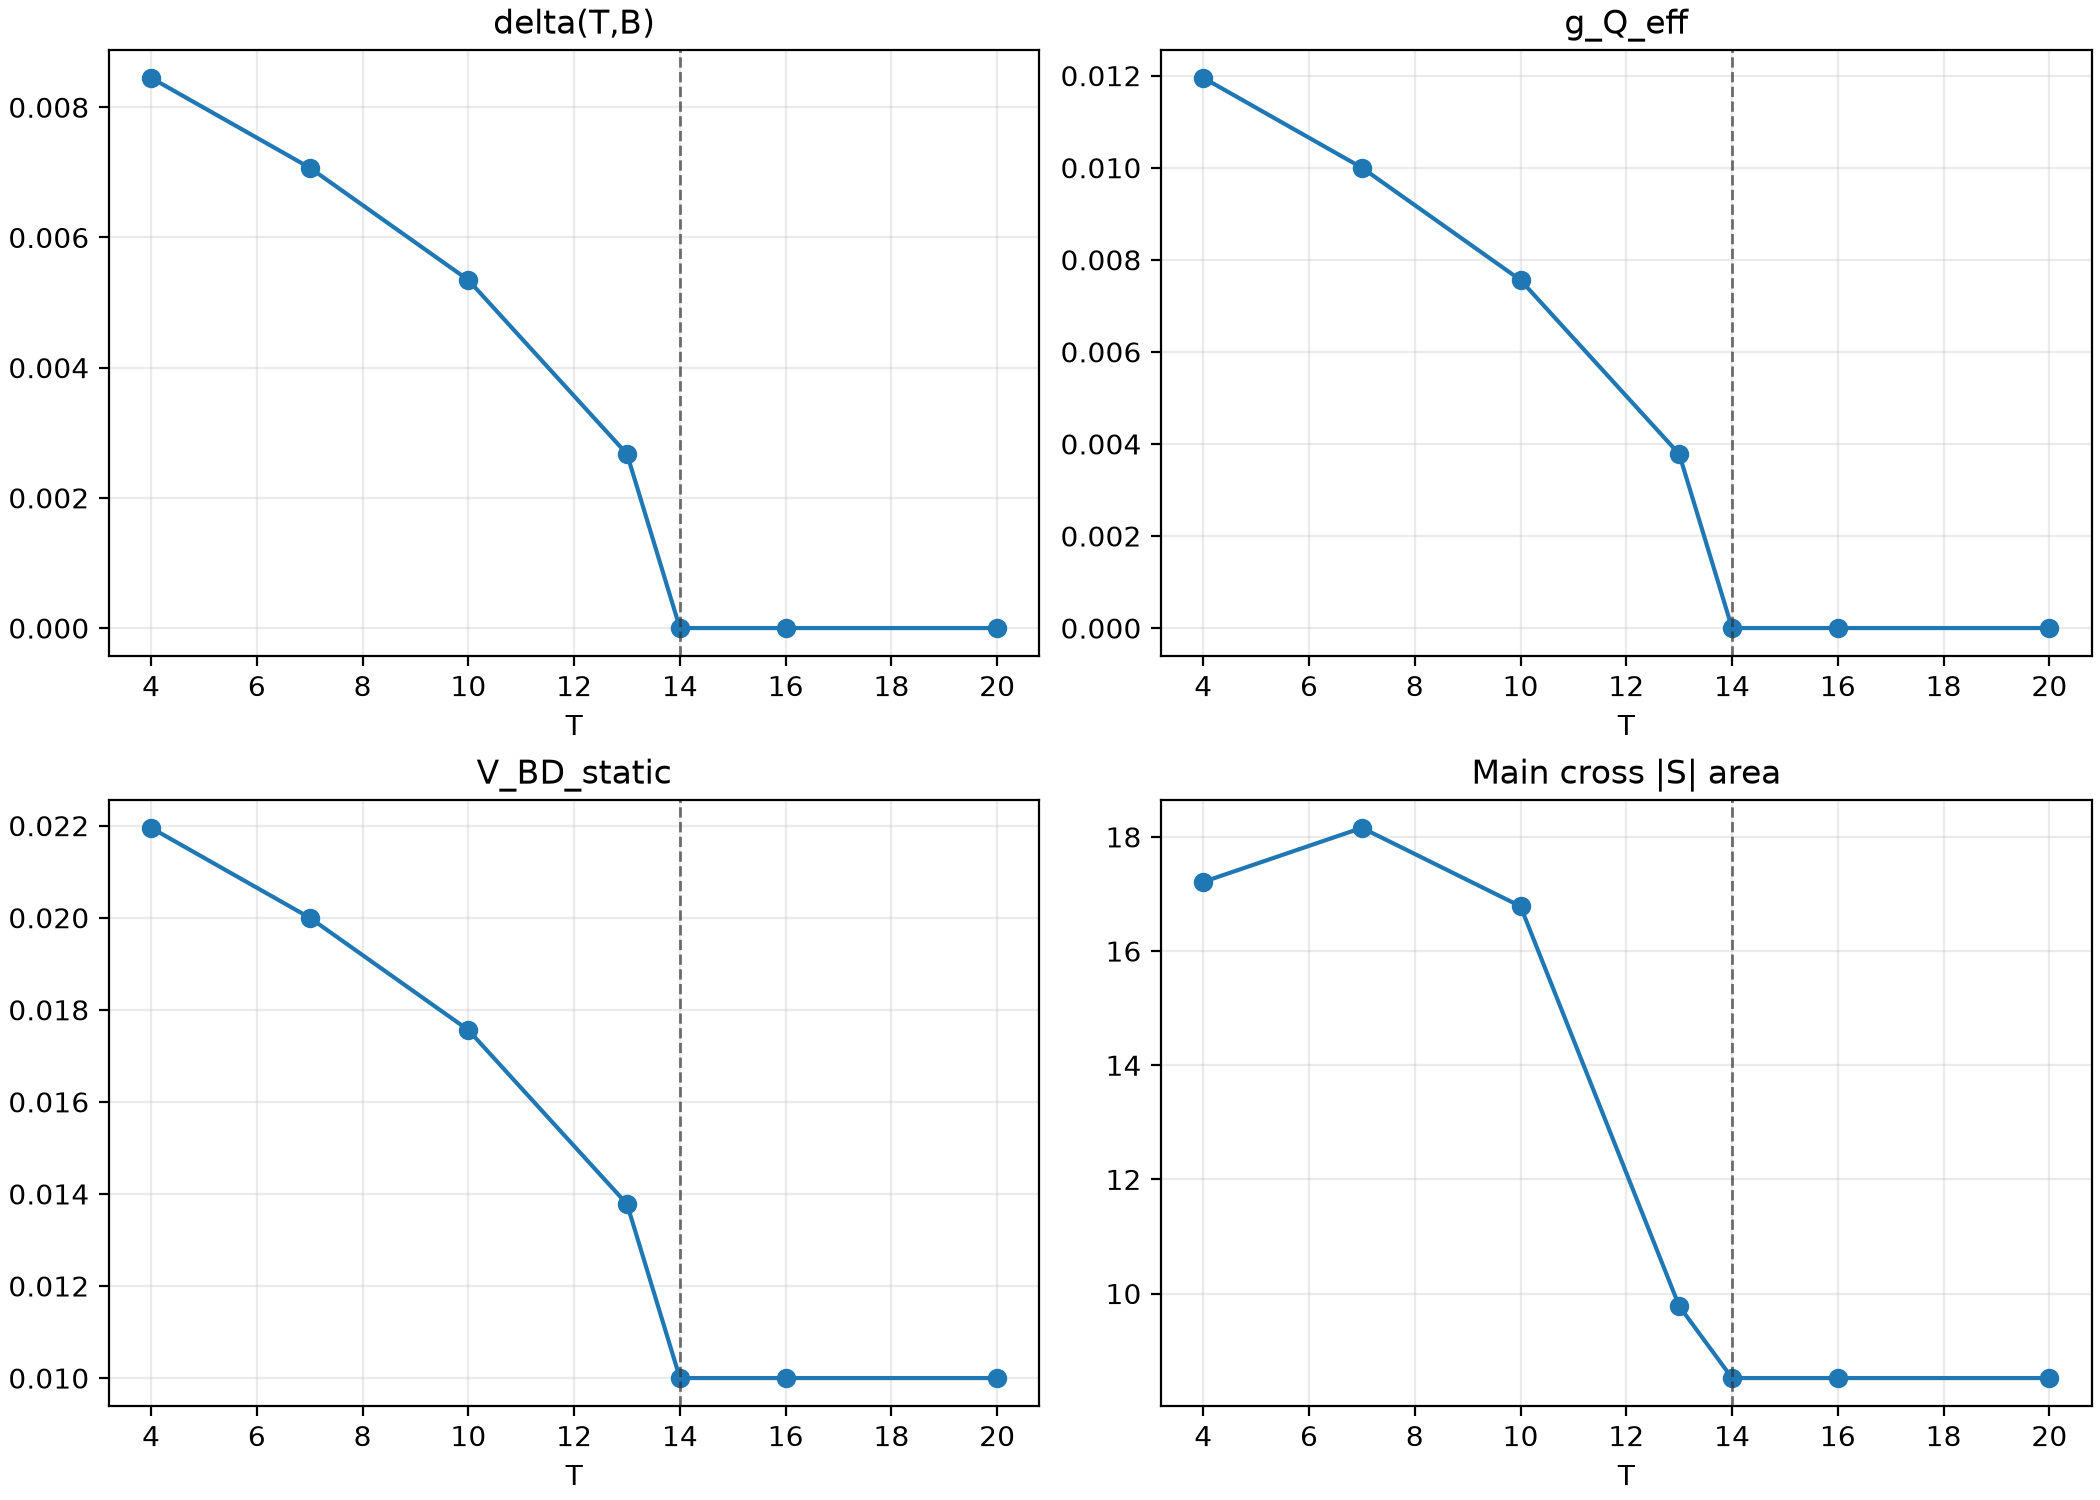
\includegraphics[width=0.95\linewidth]{Analysis/step5_temperature_lattice_dynamic_trend.png}
\caption{Temperature scan for the dynamic lattice channel.  The vertical dashed
line marks $T_{\mathrm{SP}}=14$.}
\end{figure}

\begin{figure}[h]
\centering
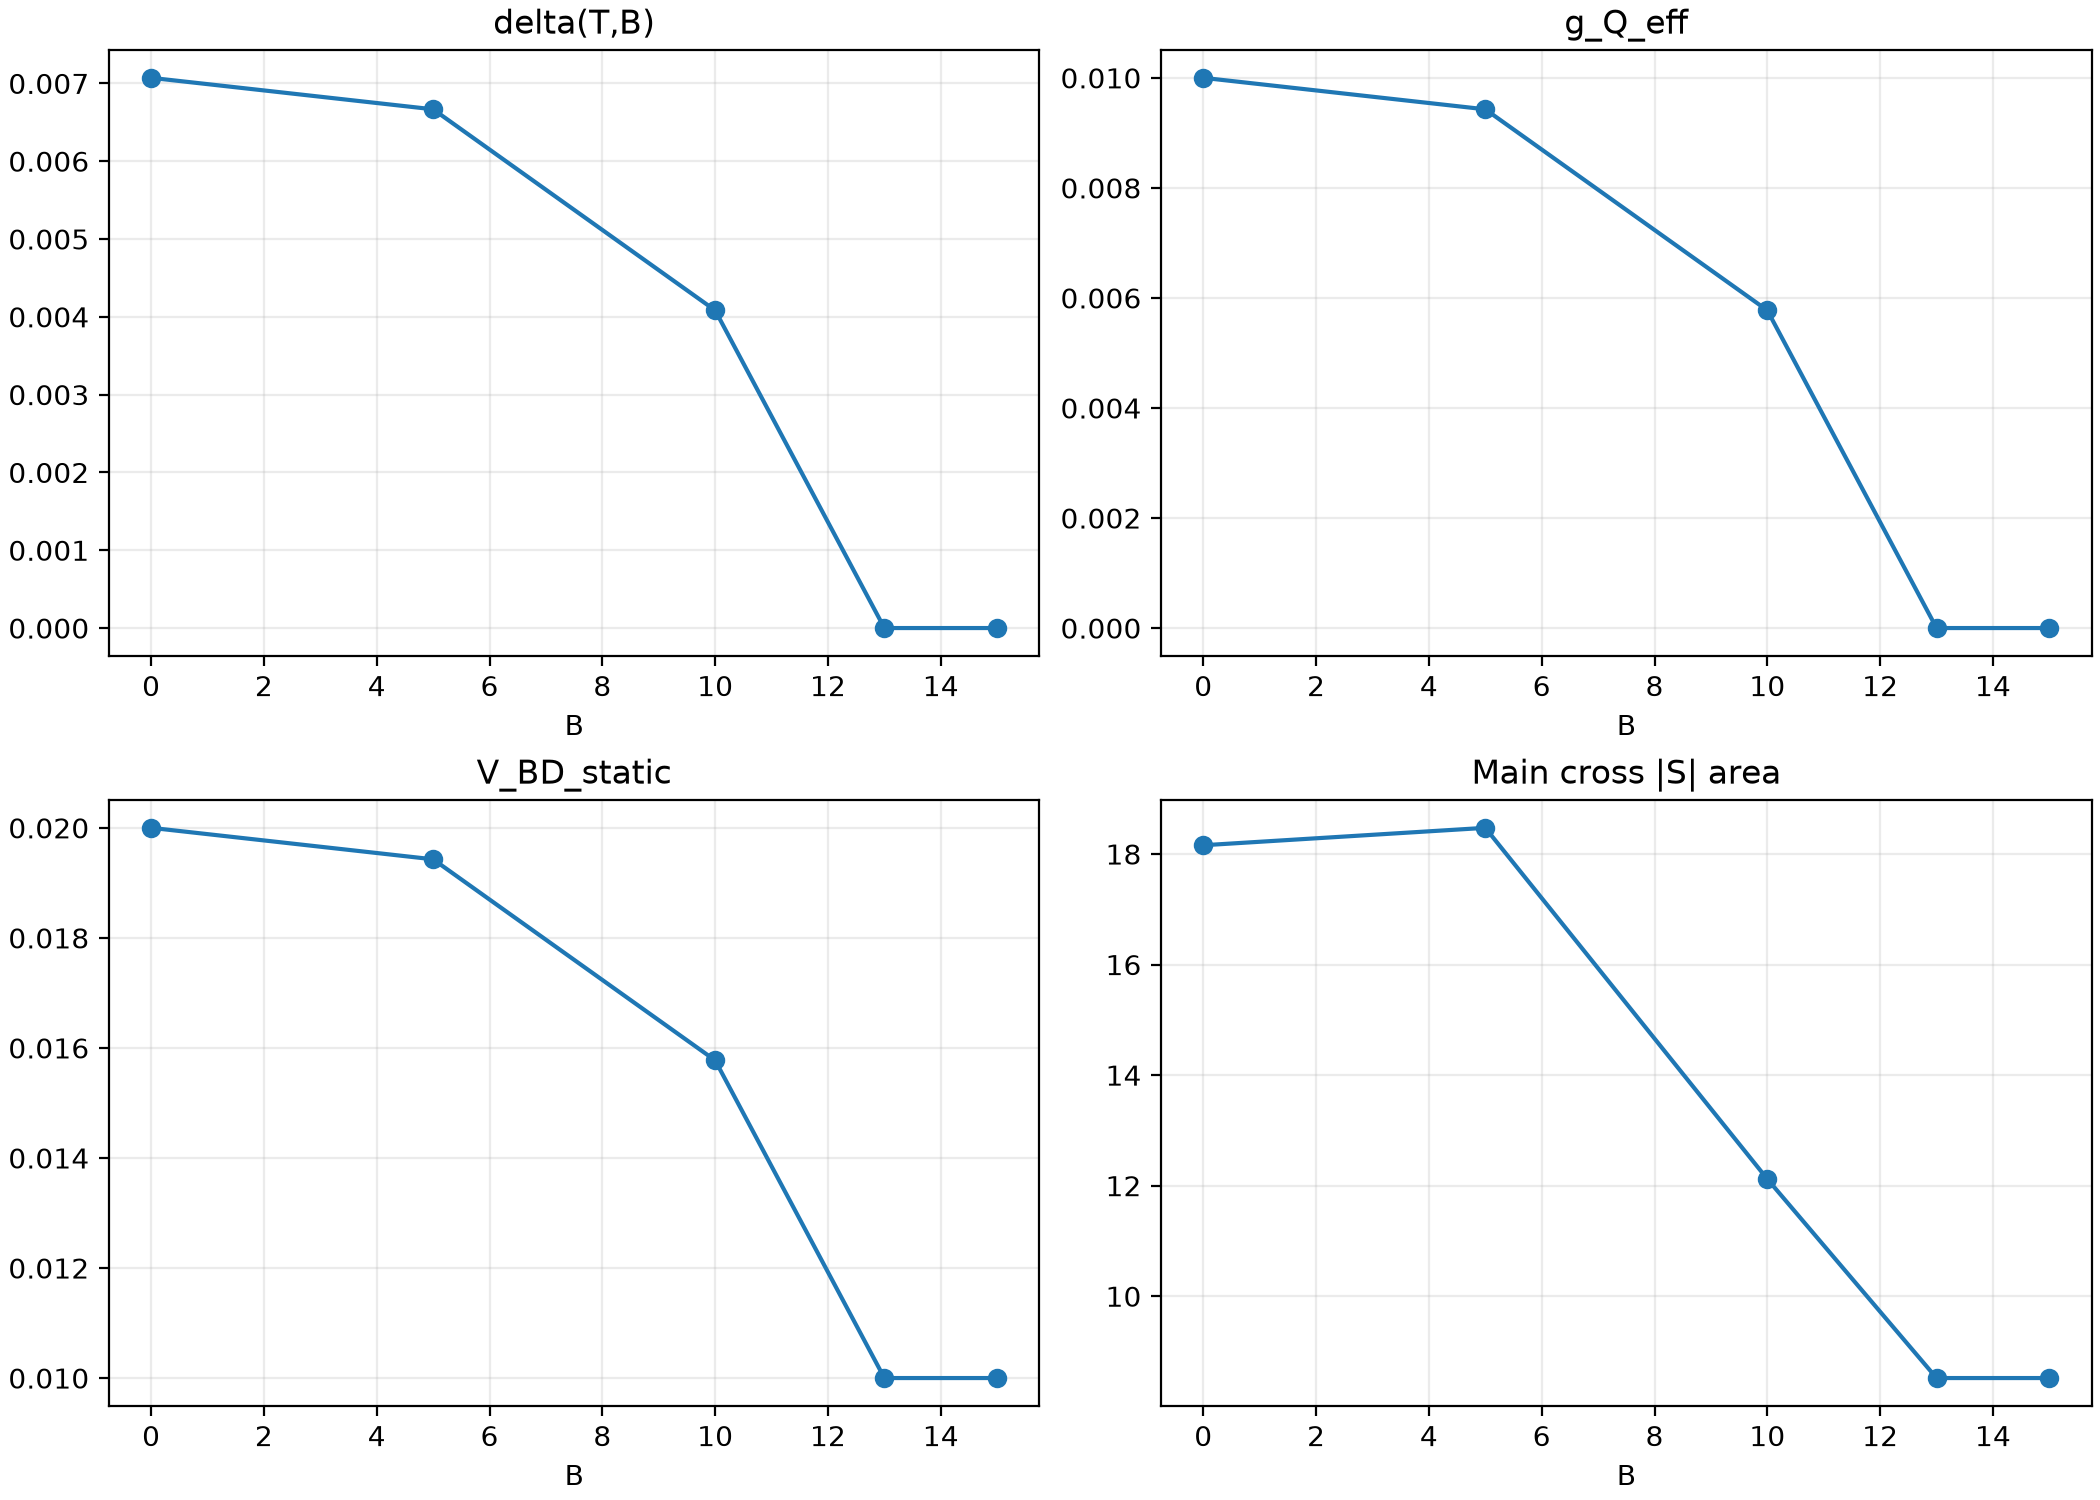
\includegraphics[width=0.95\linewidth]{Analysis/step5_field_lattice_dynamic_trend.png}
\caption{Field scan at fixed $T=7$.  The lattice channel is suppressed once
$T_{\mathrm{SP}}(B)$ falls below the fixed temperature.}
\end{figure}

\begin{figure}[h]
\centering
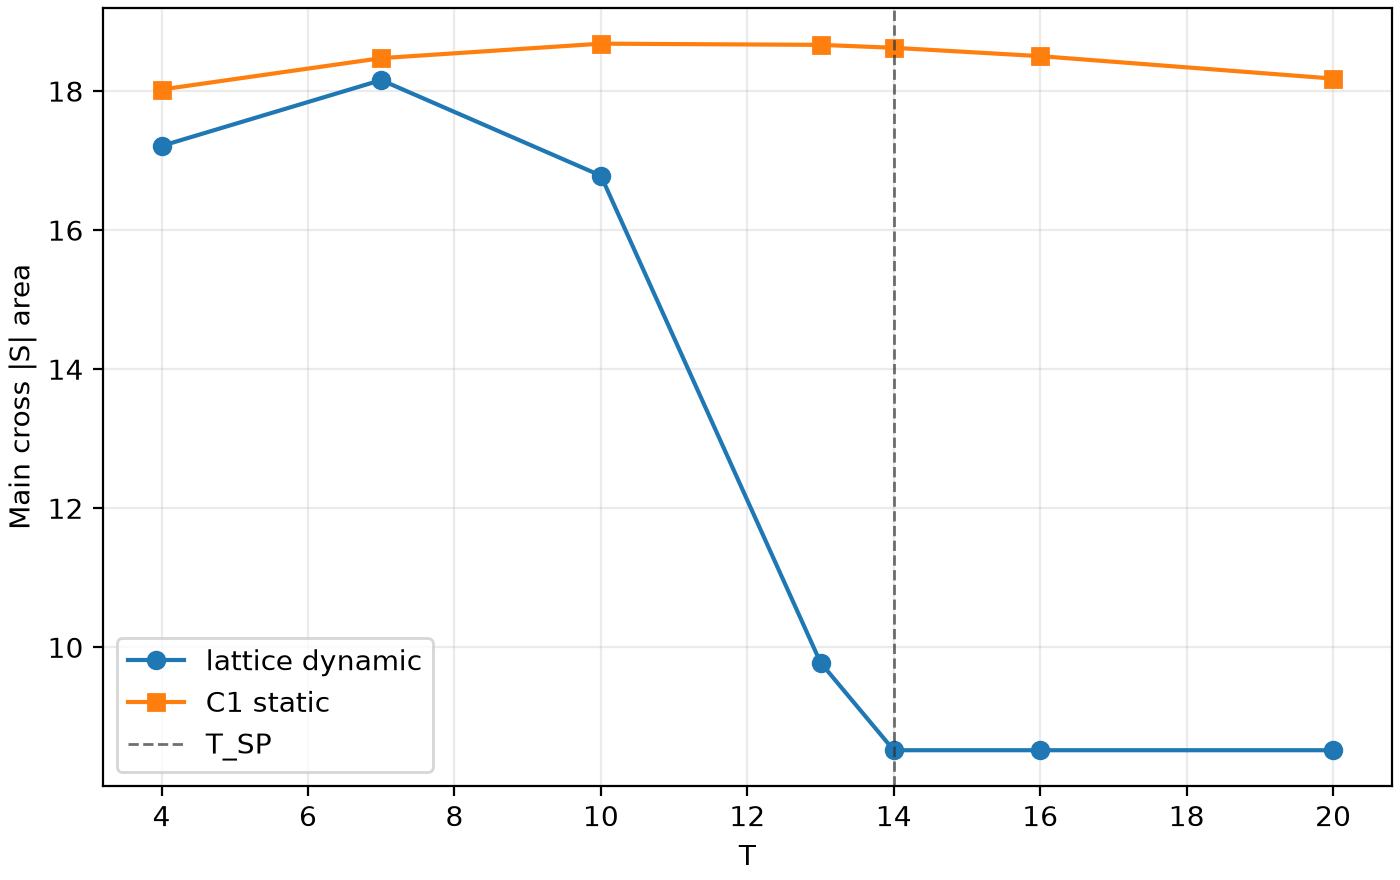
\includegraphics[width=0.78\linewidth]{Analysis/step5_temperature_lattice_vs_C1.png}
\caption{Temperature comparison between the dynamic lattice channel and the
static $C_1$ control.}
\end{figure}

\section{Validation outcome}
The Step 5 scan validates the trend-level interpretation.  The dimerisation
$\delta(T,0)$ decreases monotonically across the temperature scan and vanishes
at and above $T_{\mathrm{SP}}$.  The dynamic lattice coupling
$g_Q^{\mathrm{eff}}$ follows the same trend.  The high-temperature lattice
endpoint therefore has both $\delta=0$ and $g_Q^{\mathrm{eff}}=0$.

The field scan also passes the control.  At fixed $T=7$, the high-field points
$B=13$ and $B=15$ suppress the spin-Peierls transition temperature below the
fixed temperature, giving $\delta=0$ and $g_Q^{\mathrm{eff}}=0$.  The
cross-window area reaches the same lattice-off value as the high-temperature
scan.

The $C_1$ static scan provides the interpretive warning.  It keeps finite
$C_1$ above the transition and gives a strong cross-window signal even when
$\delta=0$.  Therefore a nonlinear feature that persists above
$T_{\mathrm{SP}}$ should not be assigned uniquely to the dimerised
spin-Peierls phase.  It may instead reflect a local spin-correlation
contribution to bright-dark mixing.

\section{Conclusion}
Step 5 turns the discrete Step 4 controls into a practical trend diagnostic.
For this minimal model, the lattice-dynamic signature follows the
spin-Peierls order parameter and collapses to a common baseline when
$\delta(T,B)$ vanishes.  The $C_1$ static control remains large across the same
temperature range.  The next useful model step is therefore not another scalar
trend control, but either a scan of the dynamical phonon parameters
$(g_Q,\omega_Q)$ or a controlled reintroduction of momentum/spinon-sector
structure.

\end{document}
